\documentclass{beamer}
% \usepackage[authoryear]{natbib}
\usepackage{graphicx}
\graphicspath{/home/evo/4m_final_project}
\usepackage{amsmath,amsthm,amssymb}
\usepackage{verbatim}
\usepackage{times}
\usepackage[sc]{mathpazo} % Use the Palatino font
\usepackage[T1]{fontenc} % Use 8-bit encoding that has 256 glyphs


%Information to be included in the title page:
\title{Multivariate analysis of the diabetes dataset}
\author{Rayyan Kazim,Safi Khan,Xinyi Chen,Tony Xu, Zesen Chen}
\institute{McMaster University}
\date{12/2/2024}

\begin{document}

\frame{\titlepage}

\begin{frame}
\frametitle{Dataset, EDA and data preparation}
\begin{itemize}
    \setlength\itemsep{1em}
    \item Using the `R` programming language, we will study the diabetes dataset obtained from Kaggle which has 768 rows and 9 columns where each row corresponds to an unique patient record. 
    \item All variables are integers except for "BMI" and "DiabetesPedigreeFunction" which are categorized as float variables.
    \item The response variable in our dataset is "outcome" and all other variables are predictor variables.
    \item 75 percent of the data will be used for training, and the rest will be used for testing.
\end{itemize}
\end{frame}

% \begin{frame}
%     \frametitle{Exploratory Data Analysis (EDA) and data preparation}
%     %insert all our tables
%     \begin{itemize}
%         \setlength\itemsep{1em}
%         \item All variables are integers except for "BMI" and "DiabetesPedigreeFunction"

%         \item The dataset will be split into 2, with the response variable being "outcome" and all other variables being predictor variables.
%         \item 75 percent of the data will be used for training, and the rest will be used for testing.
%     \end{itemize}
% \end{frame}

\begin{frame}
    \frametitle{Exploratory Data Analysis (EDA) and data preparation}
    \begin{figure}[h!]
        \centering
        % First figure
        \begin{minipage}{0.45\textwidth}
            \fbox{{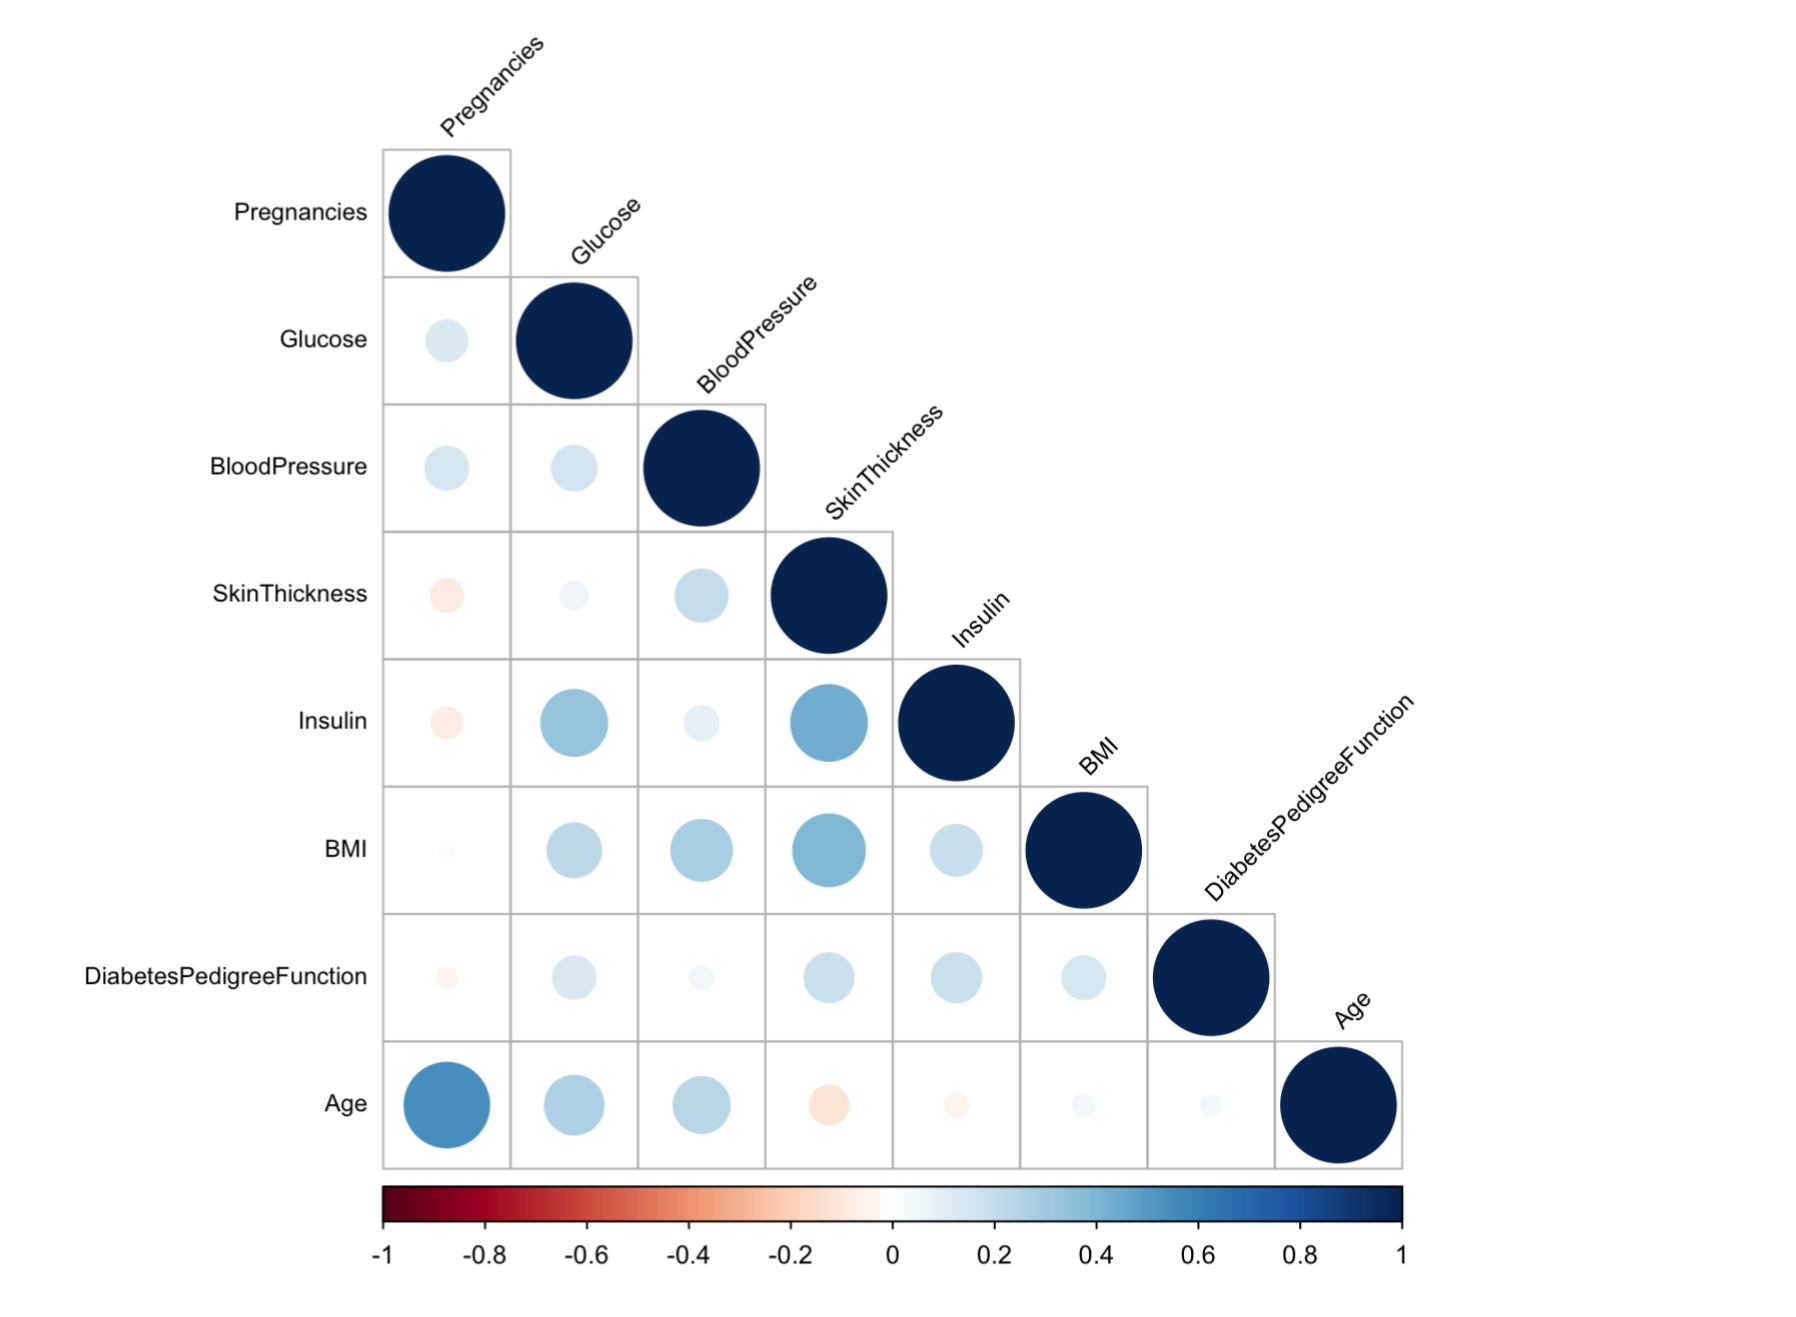
\includegraphics[width=\textwidth]{correlations2.png}}}
            \caption{Correlation of Variables} 
            \label{fig:corplot}
        \end{minipage}
        \hfill % Horizontal space between figures
        % Second figure
        \centering
        \begin{minipage}{0.45\textwidth}
            \centering
            \fbox{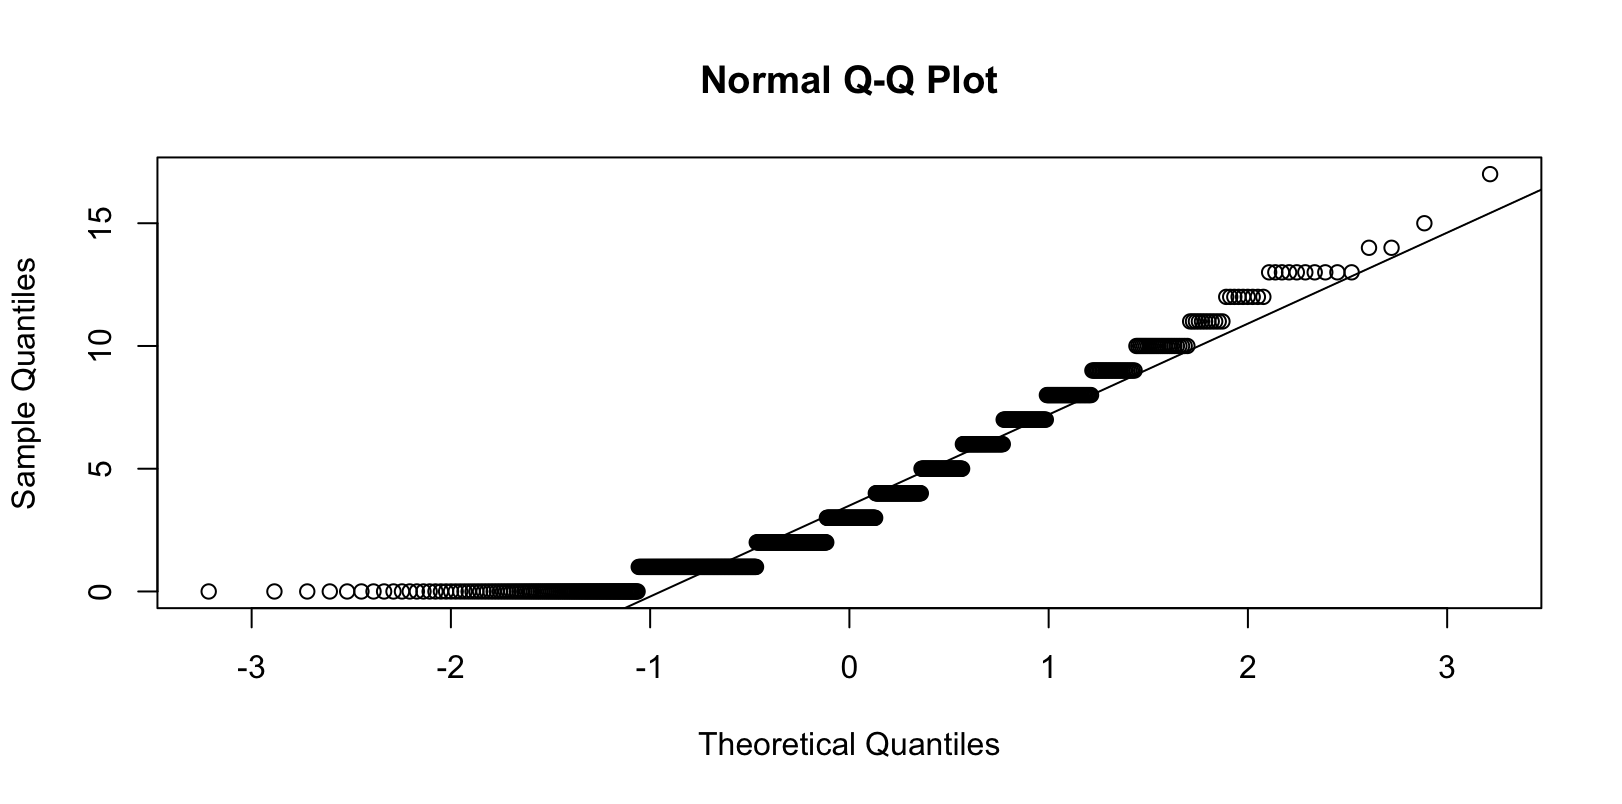
\includegraphics[width=\textwidth]{normal.png}} 
            \caption{Normal QQ-Plot} 
            \label{fig:qqplot}
        \end{minipage}
    \end{figure}
    \begin{itemize}
        \item The normal QQ-plot suggzests that our dataset is not normal
        \item SkinThickness" is well correlated with "BMI" and "Insulin", "Age" is well correlated with "Pregnancies".
        \item "Glucose" is reasonably correlated with "insulin", "BMI" and "Age".
    \end{itemize}
    
\end{frame}

\begin{frame}
    \frametitle{Methodologies - Supervised learning analysis}
        \begin{itemize}
            \setlength\itemsep{1em}
            \item We used the methods: k-nearest neighbours ,random forest classfiers and boosting for our supervised learning analysis.
            \item K-nearest neighbours is a non-parametric, supervised learning classifiers that uses proximity to make classifications about the grouping of a dataset.
            \item RandomForest classifiers is a bootstrapping sampling method that combines the results of multiple decision trees to draw on a conclusion.
            \item Boosting is similar to random forest, however it is not a bootstrapping sampling method. Boosting also uses the entire dataset, or some subsample thereof, to generate the ensemble.
        \end{itemize}
\end{frame}

\begin{frame}
    \frametitle{Methodologies - Logistic regression}
        \begin{itemize}
            \setlength\itemsep{1em}
            \item We will perform a binary logistic regression since our response variable "outcome" is binary.
            \item The initial model incorporates all eight predictor variables.
            \item The objective of this technique is to identify the most significant predictor using backwards elimination.
            \item We want the final model to have only the most significant variables. Removed predictors with p-values > 0.05.
        \end{itemize}
\end{frame}

% \begin{frame}
%     \frametitle{Discussions - Logistic regression}
%         \begin{itemize}
%             \setlength\itemsep{1em}
%             \item Table ~\ref{tab:BinLogReg} suggests that we should remove variables "SkinThickness" and "insulin" from the model, since their p-values were greater than $0.05$.
%             \item Table ~\ref{tab:BinLogRegA} implies that we have sufficient evidence to suggest that "Pregnancies", "Glucose", "Blood Pressure", "BMI", "DiabetesPedigreeFunction" and "Age" have a significant influence over "outcome". 
%             \item We obtain that the MCR for binary logistic regression is $0.23958$.
%         \end{itemize}
% \end{frame}

\begin{frame}
    \frametitle{Discussions - Logistic regression}
        \begin{itemize}
            \setlength\itemsep{1em}
            \item Table ~\ref{tab:BinLogReg} suggests that we should remove variables "BloodPressure", "SkinThickness", "insulin", and "Age" from the model, since their p-values were greater than $0.05$.
            \end{itemize}
 \begin{table}[h!]
        \centering
        \resizebox{=0.75\textwidth}{!}{
            \begin{tabular}{|l|l|l|l|l|}
                \hline
                \textbf{Coefficients} & \textbf{Estimate} & \textbf{Std. Error} & \textbf{Z-Value} & \textbf{Pr(>|Z|)} \\ \hline
                (Intercept) & -0.863576 & 0.111504 & -7.745 & 9.57E-15 \\ \hline
                Pregnancies & 0.411598 & 0.128257 & 3.209 & 1.33E-03 \\ \hline
                Glucose & 1.003291 & 0.133428 & 7.519 & 5.51E-14 \\ \hline
                BloodPressure & -0.15522 & 0.122145 & -1.271 & 0.2038 \\ \hline
                SkinThickness & -0.008376 & 0.123519 & -0.068 & 0.94594 \\ \hline
                Insulin & -0.160385 & 0.120504 & -1.331 & 1.83E-01 \\ \hline
                BMI & 0.699525 & 0.135793 & 5.151 & 2.59E-07 \\ \hline
                DiabetesPedigreeFunction & 0.295516 & 0.114215 & 2.587 & 0.00967 \\ \hline
                Age & 0.212147 & 0.127142 & 1.669 & 0.0952 \\ \hline
            \end{tabular}
        }
        \caption{Binary Logistic Regression Full Model Output}
        \label{tab:BinLogReg}
    \end{table}    
\end{frame}
\begin{frame}
    \frametitle{Discussions - Logistic regression}
    \begin{itemize}
        \item Table~\ref{tab:BinLogRegA} implies we have sufficient evidence to suggest those four variables have a significant influence over "outcome".
    \end{itemize}
    \begin{itemize}
        \item Odds Ratio show the influence of various factors on the likelihood of developing diabetes
    \end{itemize}
    \begin{table}
        \centering
        \resizebox{=\textwidth}{!}{
            \begin{tabular}{|l|l|l|l|l||l|}
                \hline
                Coefficients: & Estimate & Std. Error & z value & Pr(>|z|) & Odds Ratio \\ \hline
                (Intercept)   & -8.118918 & 0.730397 & -11.116 & <2e-16 & --- \\ \hline
                Pregnancies   & 0.154186  & 0.032151 & 4.796   & 1.62E-06 & 1.167 \\ \hline
                Glucose       & 0.030679  & 0.003781 & 8.113   & 4.92e-16 & 1.031 \\ \hline
                BMI           & 0.080086  & 0.016048 & 4.990   & 6.03e-07 & 1.083 \\ \hline
                DiabetesPedigreeFunction & 0.863621 & 0.336274 & 2.568 & 0.0102 & 2.372 \\
                \hline
            \end{tabular}
        }
        \caption{Binary Logistic Regression Reduced Model Output with Odds Ratio}
        \label{tab:BinLogRegA}
    \end{table}
    \begin{itemize}
        \item We obtain that the MCR for binary logistic regression is $0.23958$.
    \end{itemize}
\end{frame}



\begin{frame}
    \frametitle{Discussions - k-nearest neighbours}
    %insert the plot here.
        \begin{itemize}
            \setlength\itemsep{1em}
            \item 5-fold cross validation suggests that the best value for $k$ is $3$.
            \item Executing the knn() function with $k=3$, we obtain that the MCR of the k-nearest neighbours is $0.2916667$
        \end{itemize}
        \begin{figure}[h!]
            \centering
            \fbox{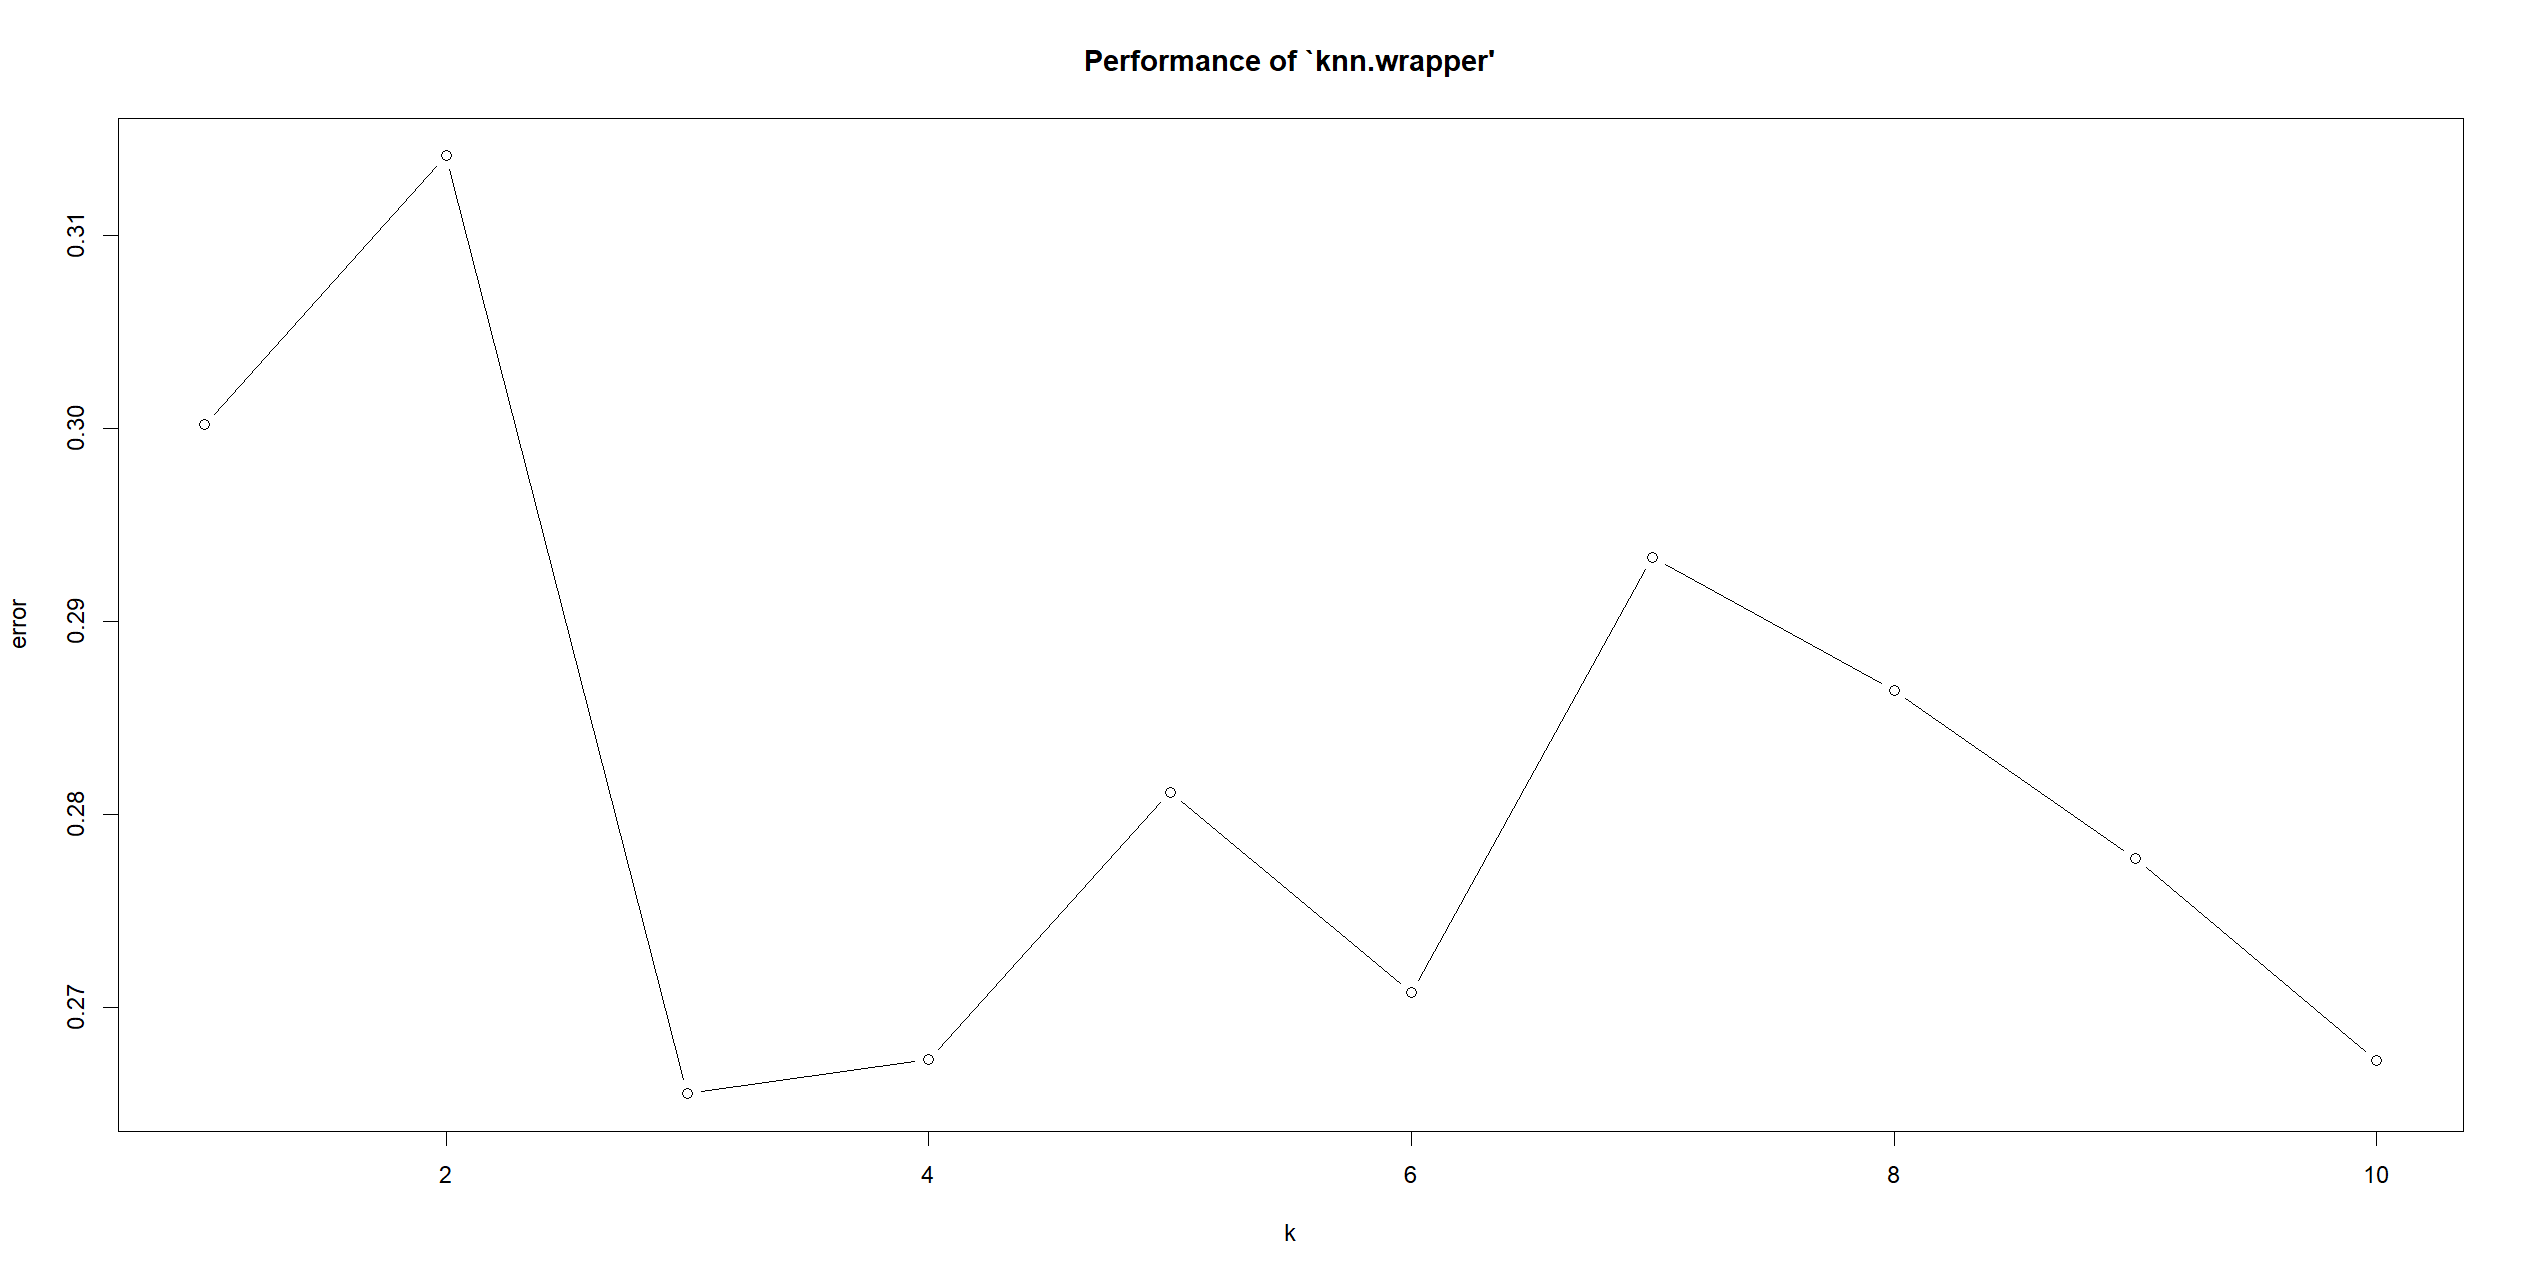
\includegraphics[width=0.80\textwidth]{knnplot.png}} 
            \caption{Output Plot From k-NN Classification} 
            \label{fig:KNNPlot}
        \end{figure}
\end{frame}

\begin{frame}
    \frametitle{Discussions - Random forests}
    %insert the variable importance plot here.
        \begin{itemize}
            \setlength\itemsep{1em}
            \item 5-fold cross validation suggests that the best value for mtry is $4$ and the best value for ntree is $200$.
            \item Executing the RandomForest()  function with mtry $=4$ and ntree $=200$, we obtain that the MCR of the RandomForest is $0.28125$.
            \item We observe that Glucose and BMI are the two most important variables.
        \end{itemize}
        \begin{figure}[h!]
            \centering
            % First figure
            \fbox{{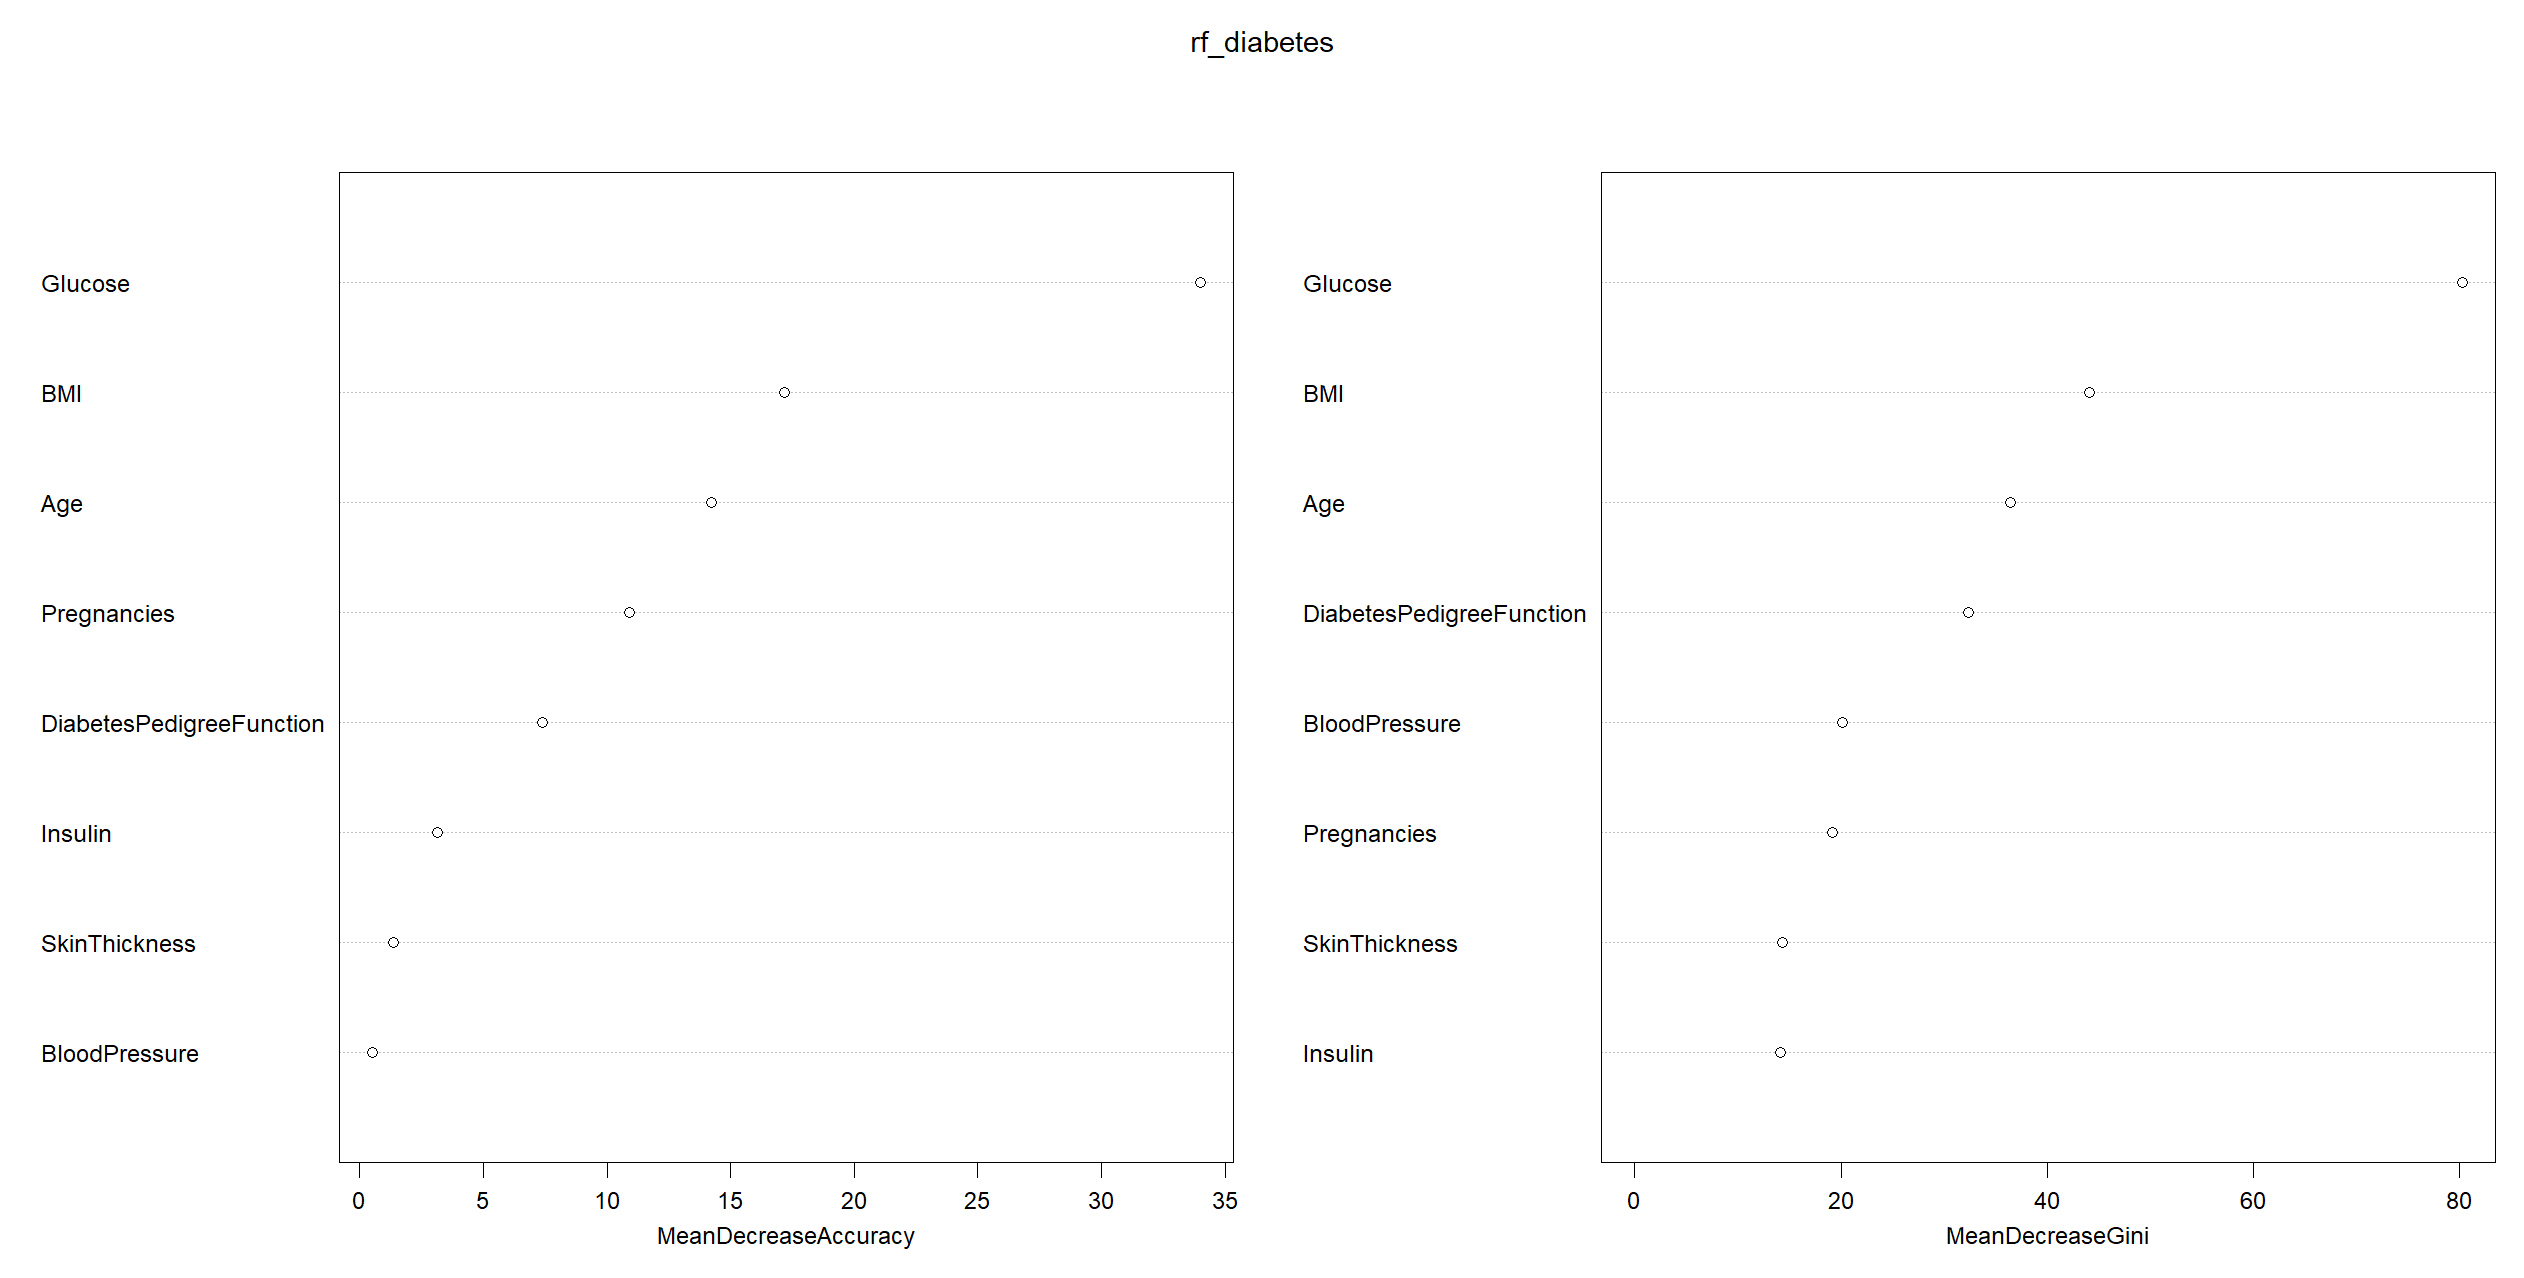
\includegraphics[width=0.50\textwidth]{MeanDecreaseAccuracyPlotForRandomForest.png}}}
            \caption{MeanDecreaseAccuracy {\&}\ MeanDecreaseGini Plot from Random Forest} 
            \label{fig:RFPlot}
        \end{figure}
\end{frame}

\begin{frame}
    \frametitle{Discussions - Boosting}
    \begin{itemize}
        \item Boosting achieved an accuracy of $73.44$ percent (a MCR of $0.2656$), with an AUC of $0.802$. 
        \item Boosting proved to be an effective method for diabetes classification through achieving an
        AUC of 0.802 and identifying Glucose, BMI, and Age as the most critical predictors.
    \end{itemize}
    \begin{figure}[h!]
        \centering
        % First figure
        \begin{minipage}{0.48\textwidth}
            \fbox{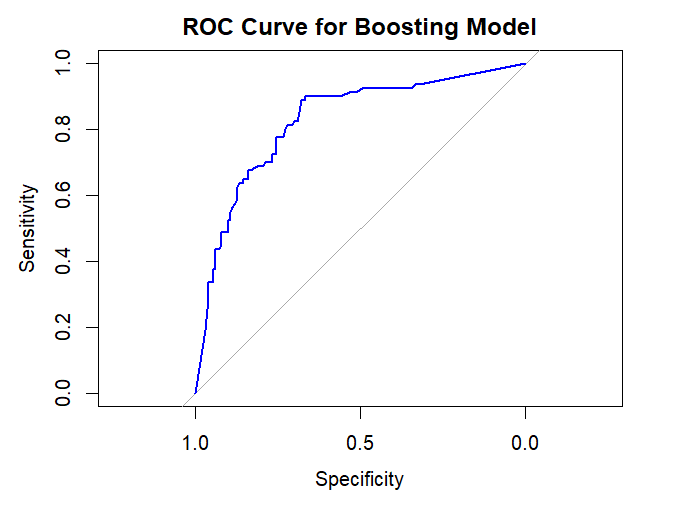
\includegraphics[width=\textwidth]{G2.png}} 
            \caption{ROC Curve for Boosting Model} 
            \label{fig:ROC curve}
        \end{minipage}
        \hfill % Horizontal space between figures
        % Second figure
        \centering
        \begin{minipage}{0.48\textwidth}
            \centering
            \fbox{{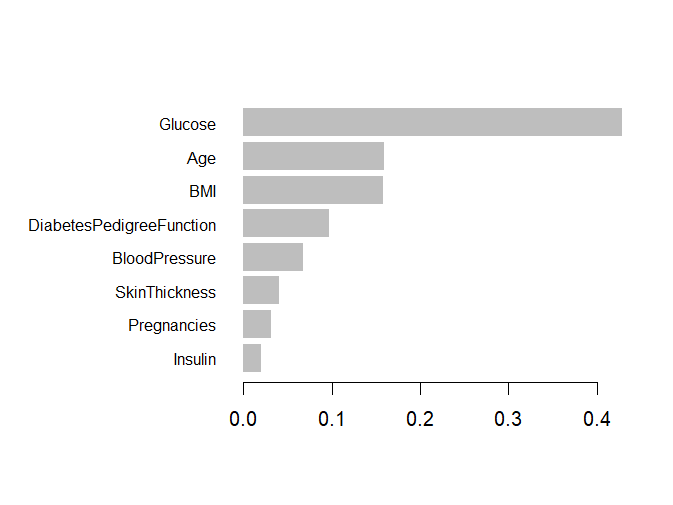
\includegraphics[width=\textwidth]{G1.png}}}
            \caption{Age Feature importance plot} 
            \label{fig:importance}
        \end{minipage}
    \end{figure}
\end{frame}
   
\begin{frame}
    \frametitle{Conclusion}
    %insert the variable importance plot here.
        \begin{itemize}
            \item The MCRs indicates that Binary logistic regression was the best method out of all methods used.
            \item We effectively showcased
            the performance accuracy of the k-Nearest Neighbours algorithm, Binary Logistic Regression al-
            gorithm, and the ensemble methods: Random Forest and Boosting. 
            \item The conclusions
            determined by each of the various methods align with the general scientific consensus on predictors for diabetes.
        \end{itemize}
\end{frame}

    % \begin{frame}
    %     \frametitle{References}
    %     \bibliographystyle{apa} 
    %     \bibliography{references}
    % \end{frame}

\end{document}
